
\chapter{Introduction}
\label{sec:INT-introduction}



\begin{flushright}
{\it The entire list of all publications
 presenting primary linguistic data \\
on Cala, Bago-Kusuntu, Phwie, Cakali
 and Pana put together \\would probably
 fit on a postcard, if back and front
 were used. }\\[2ex]

\Source{\citet[44]{Klei97}}

\end{flushright}





\section{Aims}
\label{sec:INT-aims}

The goal of the present study is two fold.  First, it  presents a broad
descriptive linguistic documentation of Chakali  by providing phonological and
grammatical preliminary studies, a bilingual lexicon and interlinearized
narrative texts. Secondly,  it describes in detail three semantic fields: 
colors, numbers and aspects of the grammatical organization of space.  

Despite the traditional presentation  grammar-lexicon-text, the originality of
the study lies in the fact that it is the first linguistic study of Chakali.  As
a result, including Chakali in Southwestern Grusi comparative, historical or
lexicographical studies is finally practicable. In addition,  the work will make
possible future systematic comparisons of Chakali and other languages using the
same robust methods, which is crucial   if both typological and comparative 
linguistics are to be taken seriously. The research also considers the
endangerment state of a
language.  By carrying out research on site for an extended period of time, I
had the chance to interact  with the community and get their opinions on the
past, present and future of their language.  Thus, the importance of documenting
Chakali  derives not only from the recent body of knowledge gathered on Grusi
languages from which Chakali is absent, but also from the  belief that the
language is in danger of disappearing.

Time constraints, training, and cultural background are responsible for
shortcomings which include   poor coverage of  the dialectal variations within
Chakali.  Therefore,   `Chakali'  here  is best defined as  `the linguistic
data
gathered by the present author in Ducie between 2007 and 2010'.  Other
deficiencies are the inadequate description of forms and functions in the verbal
domain,  of prosody at many levels as well as  the absence of basic discourse
characteristics beyond the sentence level.



Presenting his view on the issue of endangered languages,  \citet[9]{Newm03}
writes that ``[t]he only way endangered languages in Africa, for example, are
going to get described is if African linguists and their African students do the
work. Otherwise it cannot be done.''. He observes, however,   that ``we find
that our African colleagues are no more qualified, no more trained, and no more
ready to undertake the task than the most abstract theoretically-oriented
linguist''  \cite[9-19]{Newm03}. Acknowledging that the situation has changed 
slightly over the past 5-10 years, the present work is the result of an
`outsider'  carrying  out field work among the Chakali; it is a description and
an analysis of some of the material collected, but personally, first and
foremost, training in fieldwork procedures.








%What do I contribute? I focus on the object. What's the object, the phenomenon?
%Argue for it. 




%Primary data, the consequence of the transfer from speech to written made and
%organize by a non-native speaker


%Ready for a documentation: orthography and 
%Ready for a comprehensive grammar: identify problems claim analysis

\section{Literature review}
\label{sec:INT-lit-rev}

The English anthropologist Jack Goody  not only  presented the first linguistic
data on the Chakali language, which consisted of a list of 38 words gathered  on
the 29th August, 1952,  in Katua \citep[33]{Good54}, but  is also responsible
for the
identification of the existence of the language and the people who speak
it.\footnote{I cannot state this with great  confidence since there may be
British and/or French colonial documents somewhere which mention `Chakali'. For
instance,  it is known that  French Captain  Binger and his
troop
attacked some of Babatu's men in  Ducie in 1897.  Binger's reports were
impossible to get hold of.}

\begin{Lquote} I do not know of any previous record 	of the existence of the
group speaking
this dialect. Although now living entirely within the administrative district of
Wa, there is in their midst the village of Kandia inhabited only by
Guang-speaking Gonjas. The chiefship of Kandia was an important office in the
Gonja political system. Either at the time of the arrival of the British
military forces or a little before, during the course of a war between the State
of Wa, allied with Bole, and the Yabumwura, the senior chief of Gonja, it fell
within the orbit of Wa. The western section of the group comprising the villages
of Chago, Bisikan and Bulinga speaks Wala, i.e. the dialect of Dagari spoken
within the State of Wa, and was certainly under the influence of the Chiefs of
Wa before the European conquest. The Chief of Bulinga, the central village of
this section, claims to have been a Kamboŋa (a semi-dependent war-chief) in
relation to Wa. The eastern group of the Chakalle speak Chakalle and seem to
have been under the suzerainty of the Gonja Chief at Kandia. This group consists
of the villages of Katua, Tosa, Sogola, Motigu, Chasia, Ducie and
Gurembele.\\
 \Source{ \citet[3]{Good54}}
 \end{Lquote}




Since its first appearance,   Chakali has been
listed in   linguistic classifications  as a member of the
Grusi sub-group of the Gur languages (see figure \ref{fig:Gur-tree}).  Grusi  as
a language cluster has
been defined and confirmed in several publications \citep{Dela12, Kohl58,
Bend65,
Mane69a, Mane69b, Klei97}.  While the term `Grusi' is associated with a language
group, the term and its spelling variants (i.e. {\it
Gurunsi}, {\it Grunshie}, {\it Gourounsi}, etc.)  have always existed in the
French and English
colonial vocabulary, but without great unanimity on its designation
\citep{Taux21, Taux24, Ratt32a, Ratt32b, Nico52, Dupe84}.


%\cite[61]{West52} under Grusi does not have Chakali but Sisaala, Vagla,
%Tampulma and Deg. (the term gur was adopted by christaller (Sprachproben aus
%dem Sudan 1889-1890) the tern voltaique is a french tradition. Chakali is not
%indicated in westerman) the term grusi was used to identify tribes and dialects


 In \cite{Bend65},  Chakali data is used to confirm the Grusi cluster. The
material, a list of 97 words, is said to have been produced by Mr. E. R.
Rowland. His notes have not been located and remain unpublished.  
\cite{Mane69a, Mane69b} reconstructs  a {\it  gurunsi commun}  based on an
average of 80 words from twenty-six Grusi languages.  He includes, however, only
36 Chakali words, all of them extracted from \cite{Bend65}.


In 1974 and 1994, sociolinguistic surveys were carried out in the Chakali area
by the Ghana Institute of Linguistics, Literacy and Bible Translation (GILLBT),
formerly Ghana Institute of Linguistics (GIL), which is the Ghanaian branch of
the Summer Institute of Linguistics (SIL). In these two surveys, the main goal
of GIL and GILLBT  was to investigate the need of Chakali language development
and to assess  Waali comprehension. The conclusions of the 1994 survey report
are discussed in section \ref{sec:SOC-gil-socio}. In spite of this interest, the
GILLBT has not yet begun activities in the Chakali communities. 

In 1999, Ulrich Kleinewillinghöfer spent a few hours in Wa with Godfrey Bayon
Tangu \citep{Klei99}. In this short period,  he  gathered 
approximately 150 words  and from them  inferred some generalizations on Chakali
nominals.

In 2001, a Brazilian  known as Pastor Ronaldo worked with two  language
consultants in order to start a vernacular literacy project. The initiative came
from the Evangelical Church of Ghana.  Two illustrated booklets were written
with  the aim of using them for adult literacy. According to the language
consultant in charge of the teaching (personal communication) 5-10 individuals
could  read with good fluency after just a few lessons. The first booklet
introduces the alphabet designed. I was unable to locate any copies of the 
booklet.  The second 20-page booklet consists of  syllables and short sentences
thematically organized.  A photocopy of the single remaining copy is now in my
possession. 

In 2005, Prof. M.E. Kropp-Dakubu spent two  days with an informant from Jayiri,
gathering general information on Chakali  \citep{Daku05}. Her intention was to
investigate the situation on site for a documentation project. Due to the
condition of the road, she did not reach villages where Chakali is spoken by all
inhabitants. The unpublished report  presents  data which was believed to be
representative of  Chakali, but which transpired to be an idiosyncratic mix of
Waali and Chakali, and some Bulengi, which is a language used by speakers in
Bulenga and surrounding villages (see section  \ref{sec:SOC-bulengi}). 


A review of the  literature shows that  the language has been known to exist
since 1954, yet very little has been written on  it and  most of what has
been written has remained unpublished.  Nevertheless, the Grusi cluster puts
Chakali in the  {\it Southwestern Grusi} group \citep{Nade89} or,  in the latest
sub-classification of Grusi,  the {\it Western Grusi} \citep{Lewi09}, together
with Winyé, Phuie, Sissala, Western Sissala, Tumulung Sissala, Pasaale, Chakali,
Tampulma, Vagla, Dɛg and Siti.\footnote{Unfortunately, Siti is not classified
anymore. The language does not appear in \cite{Nade89} and has been relegated as
an alternate name for Vagla in \cite{Lewi09}. However, \cite{Klei99b}
re-confirms that Siti is a distinct member of the
 Western subgroup of Grusi.} Most of these languages are also poorly documented
\cite[see][]{Klei97}. 

Finally, there are studies outside linguistics by individuals who deserve to be
mentioned:  Dr. Henry Seidu Daannaa,   a native Chakali from Tuosa,  presents a
retrospective study of the practice of indirect rule system which affected the
social and political organization of  Chakali during the colonial administration
\citep{Daan94}.   Dr. Cesare Poppi conducted anthropological research which
focuses on issues related to knowledge, secrecy and initiation \citep{Popp93}
and  theoretical issues concerning the analysis of the representational status
of masks, particularly the {\S sigmaa} masks which are cornerstones of Chakali
system of beliefs.  Other sources of non-linguistic  information on Chakali can
be found in \cite{Doug66, Wilk89, Sali08},  three  publications  which deal with
Wa town and its surroundings. 


\section{Method}
\label{sec:INT-method}


Every year from 2007 to  2010, I carried out a field trip to the Wa East
district of Ghana. The longest period  was 6 months and the shortest was 2
months. Approximately 80\% of the periods were spent in a Chakali speaking
village. The linguistic data was gathered mainly in Ducie, although during these
periods I had several overnight stays in Motigu, Gurumbele and Wa, and a few day
trips to Katua and Sogla. Basic sociolinguistic surveys were conducted in Katua,
Motigu, Sogla, Ducie and Gurumbele.  



Different elicitation techniques were used.  Most natural audio-recorded data
comes from  transactions at the market, meetings with the elders,  and
interviews with commoners. Least natural are pieces of translation work using,
for instance, questionnaire 6 of \citet[257-270]{Bouq92},  or exchanges of
information with consultants of the type `how do you say X', where X stands for
an intended entity or proposition, using English as the medium of communication.
Translations from English to Chakali and from Chakali to English  were performed
mainly by four language consultants; Daniel Kanganu Karija (male, 56 Y.O.,
Ducie), Awie Bakuri Ahmed (male, 29 Y.O., Gurumbele), Fuseini Mba Zien (male, 52
Y.O., Ducie), and Afia Kala Tangu (female, 32 Y.O., Ducie). Since I do not
have linguistic competence in Chakali  their assistance was essential in 
allowing the research to progress responsibly. 


In the middle of this naturalness scale is one method of elicitation  which 
consisted of having a significant number of native speakers interpreting,
identifying and expressing perceived stimuli.  Stimulus-based data collection
has the advantage of being free from interference and provides the researcher
with a level of authenticity unattainable in (bilingual) elicitation of
paradigms
and wordlists.  In addition, the sessions and output of stimulus-based data
collection are always  controlled, quantifiable and comparable, as opposed to
the
collection of texts of different genres. Since the data collection was carried
out with several individuals, the degree of consensus within the responses can
be interpreted as signaling core, secondary or `accidental'
meaning. The same method  turned out to be useful in practical lexicography work
when the discovery procedure involved  taxonomies unknown to the researcher. For
instance, the domain of animals and plants required the identification of
species and their associated sound patterns. A problem arose when the visual
access to some species, e.g.   hyenas or seasonal plants,  was practically
impossible. Still, in the current lexicon, many species were identified using
illustrations. One disadvantage often encountered with this approach to lexicon
and
grammar discovery is that standard stimuli are no better than 
``semantically-neutral'' wordlists, e.g. Swadesh-100, since the researcher
still faces
the problem  of cross-cultural applicability.  Typically, in the context of a
village in Northern Ghana, unfamiliar items or scenes depicted may cause
disagreement in
the overall description.  These
problems are discussed in chapters \ref{sec:COL-chap} and \ref{sec:SPA-chap},
but when several individuals participate in  stimulus-based
experiments, the level of unpredictability  decreases.
Another obstacle is that pictures and illustrations may lack 
elementary features
which are crucial for
 the identification of a species (e.g. texture, odour, size, etc.). For
instance,
because  only  illustrations and pictures were used (those in \cite{Cans61,
Trap06}),  arriving at a consensus when identifying  species
of snake has proved difficult. On a more general note,  the problem with a
purely onomasiological
approach to language
description is that a concept is always depicted by   researchers, not by
the native speakers themselves. Nonetheless, studying the linguistic encoding of
predefined conceptual domains is a practice which has influenced the direction
of  a series of typological studies \cite[among others,][]{Berl69, Levi03,
Hasp03, Bohn07a, Vanh08a}. The findings in chapters \ref{sec:COL-chap},
\ref{sec:NUM} and \ref{sec:SPA-chap} are based on the study of three semantic
domains and subscribe to that line of research. 

\subsection{Softwares}
\label{sec:INT-software}

6 short stories, 30 proverbs, 20
interviews and 18  songs were recorded and transcribed on site. The majority
were
audio recorded, whereas all songs, 3 stories and  a few market transactions 
were
video recorded. The texts are managed and semi-analyzed using three kinds of
software. 
The Field Linguist’s Toolbox\footnote{http://www.sil.org/computing/toolbox/}
encodes the text data. It uses a text database that has a fixed format, but no
predefined fields. The transcription employs the orthography described in
chapter \ref{sec:chap-phono}, which is a Latin alphabet supplemented with
symbols
from International Phonetic Alphabet.   Since the  full interlinearization of a
text is time-consuming,  only  a few of them are entirely
interlinearized. Two interlinearized texts are presented in the appendix
(page 
\pageref{chap:TXT-text}).   The same software  manages the lexical data. The
dictionary and index of  chapter \ref{sec:LEX-lexicon} is extracted from a
bilingual Chakali-English database  containing more than 2100 Chakali headwords.
It has been processed and exported  by another of  SIL's softwares, i.e. Lexique
Pro.\footnote{http://www.lexiquepro.com/}  Dekereke, a phonology software
designed by Rod Casali,\footnote{http://casali.canil.ca/}
systematically identifies  the phoneme inventory,  syllable structures and
minimal
pairs, among other things.

\subsection{Conventions}
\label{sec:INT-gloss}


The glossing tags presented on page  \pageref{sec-ABB} are for the most part
equivalent to the conventions designed in \cite{Lehm82} and \cite{Comr08b}.  As
a rule,   a three-line morpheme-by-morpheme  glossing for textual
data is provided, but  four lines may exceptionally appear. 


\begin{exe}
\ex\label{ex:INT-pre-adj}
\gll tʃʊ̀ɔ̀sá  pɪ̀sɪ̀   à    bìpɔ̀lɪ́ɪ̀  kpá ʊ̀ páŕ\\ 
morning   scatter   {\art} young.man take {3\sg.\poss} hoe\\
 `The following day the young man took his hoe along ...' (CB story 5)
\end{exe}


 The first line is a representation of the object language, the second line
consists of   tags representing  rough approximations   of the morpheme in the
object   language
 (e.g. function, meaning, part-of-speech), whereas the third line is a
free  translation capturing the general meaning  conveyed in the object
language's line.  The use of capital letters in the  free translation
corresponds to a focused constituent. The non-overt expression of a feature is
enclosed within round brackets following the Leipzig glossing rules
\citep{Comr08b}. An interlinearized example  may  be accompanied by a
reference  to a particular text or  a situation in which  the utterance was
collected, as shown in  (\ref{ex:INT-pre-adj}).

It is admitted that tone is not consistently marked. At this stage,  the
transcription and description of tone will require an analysis of
considerable sophistication, something which deserves a separate study. 
The convention for marking tone we use in this thesis is; high (  ́) and
low (  ̀). Tone and intonation are treated in section
\ref{sec:tone-intonation}.










%because
% Among the thirteen villages forming 
% Chakali land, only four villages are believed  by the population  to be
%villages
% where Chakali is spoken by the majority (i.e. Motigu, Gurumbele, Ducie and
% Katua). This
% impression is shared in Gurumbele, Sogla, Motigu and Ducie among the elders
% and youth. When meeting with the council of elders in Sogla, Motigu, Ducie
%and
% Bele, we regularly hear that in a period of less than
% 70 years the Chakali
% people lost a great deal of their traditional authorities (legal system), due
%to
% the coalition British-Wala,  a considerable amount of their hunting
% land and a given away their language. 




\section{Organization of the chapters}
\label{sec:INT-organis-of-chap}


The thesis is divided into nine chapters. Chapter \ref{sec:SOC-lingvit} presents
an overview of the sociolinguistic situation. The degree of endangerment of the
language is assessed,  based on the criteria set up in \cite{Reco03}.  Why
Chakali is treated as an endangered language,  and why Chakali is still spoken
today  are the main questions. Chapter \ref{sec:chap-phono} presents an outline
of the phonology based almost entirely on a lexical database. Since one cannot
describe anything systematically without some theoretical assumption,  the set
of (articulatory) features proposed in \cite{Lade07} is assumed. Chapter
\ref{sec:gramsketch} provides a grammar outline based on a lexical database,
transcribed texts and output of controlled elicitation. The grammar adopts a
framework relevant for typology and language description, such as the `basic
linguistic theory' of \cite{Dixo10a, Dixo10b}.  Also, the approach to
description proposed in  \cite{Bonv88} on Kasem,
\cite{Mcgi99} on Pasaale,  and \cite{Nade98} on Vagla have proven to be  useful
references for understanding some obscure issues. Chapters \ref{sec:COL-chap}, 
\ref{sec:NUM} and  \ref{sec:SPA-chap} describe how Chakali encodes three
semantic domains  and investigate which systems (i.e. lexical, morphological,
syntactic, prosodic)  express which meanings. Chapter \ref{sec:COL-chap} deals
with color terms. The elicitation techniques suggested in \cite{Davi95} are
employed and the language  is assigned to the typological and evolutionary
scheme of \cite{Kay99}. Chapter \ref{sec:NUM} describes the numeral system in
detail. It is followed by a digression into comparative linguistics,  which
suggests  a Southwestern Grusi clustering  based on the numerals of five
languages.  Employing five elicitation techniques, chapter  \ref{sec:SPA-chap}
reveals Chakali's basic locative construction \cite[15]{Levi06} and  subscribes
to the typology of locative predicates proposed by \cite{Amek07b}. Chapter
\ref{sec:LEX-lexicon} contains  a Chakali-English dictionary and an
English-Chakali glossary. Finally, the appendix (page \pageref{chap:TXT-text}) 
presents two folktales  interlinearized with  a four-line morpheme-by-morpheme
glossing and a translation. 

 \begin{sidewaysfigure}
 \centering
 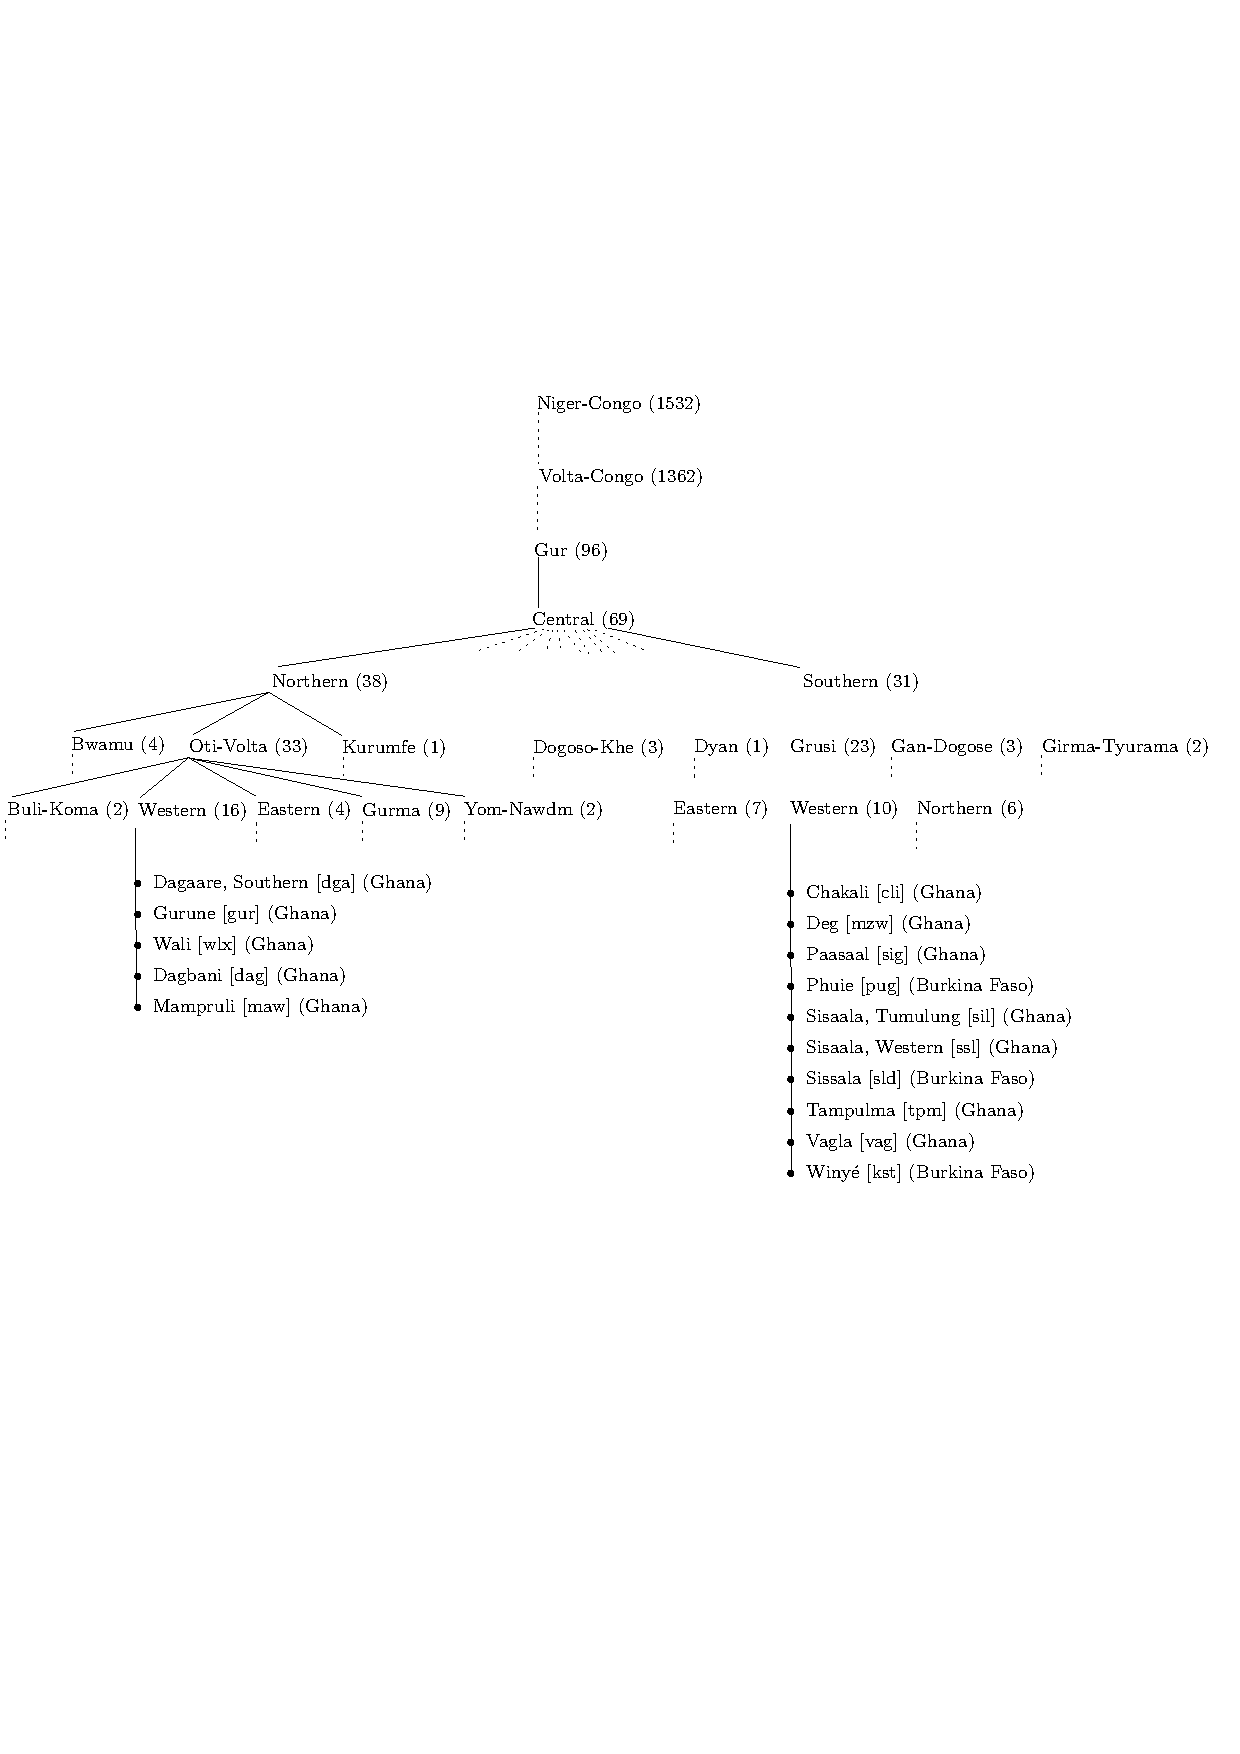
\includegraphics[width=15cm,height=10cm]{Graphic/Pictures/Gur-tree.pdf}
  \caption[Gur groups and clusterings]{Some Gur groups and clusterings.
Number of languages in a cluster and country where the languages are
spoken are included in
parenthesis. The ISO 639-3 code letters appear within square brackets.
All Western Grusi and the Western Oti-Volta mentioned in this work are
displayed. Names of languages and clusters as appearing  in 
\cite{Lewi09}
\label{fig:Gur-tree}}
\end{sidewaysfigure}

\newpage


\begin{figure}[htp]
\centering
%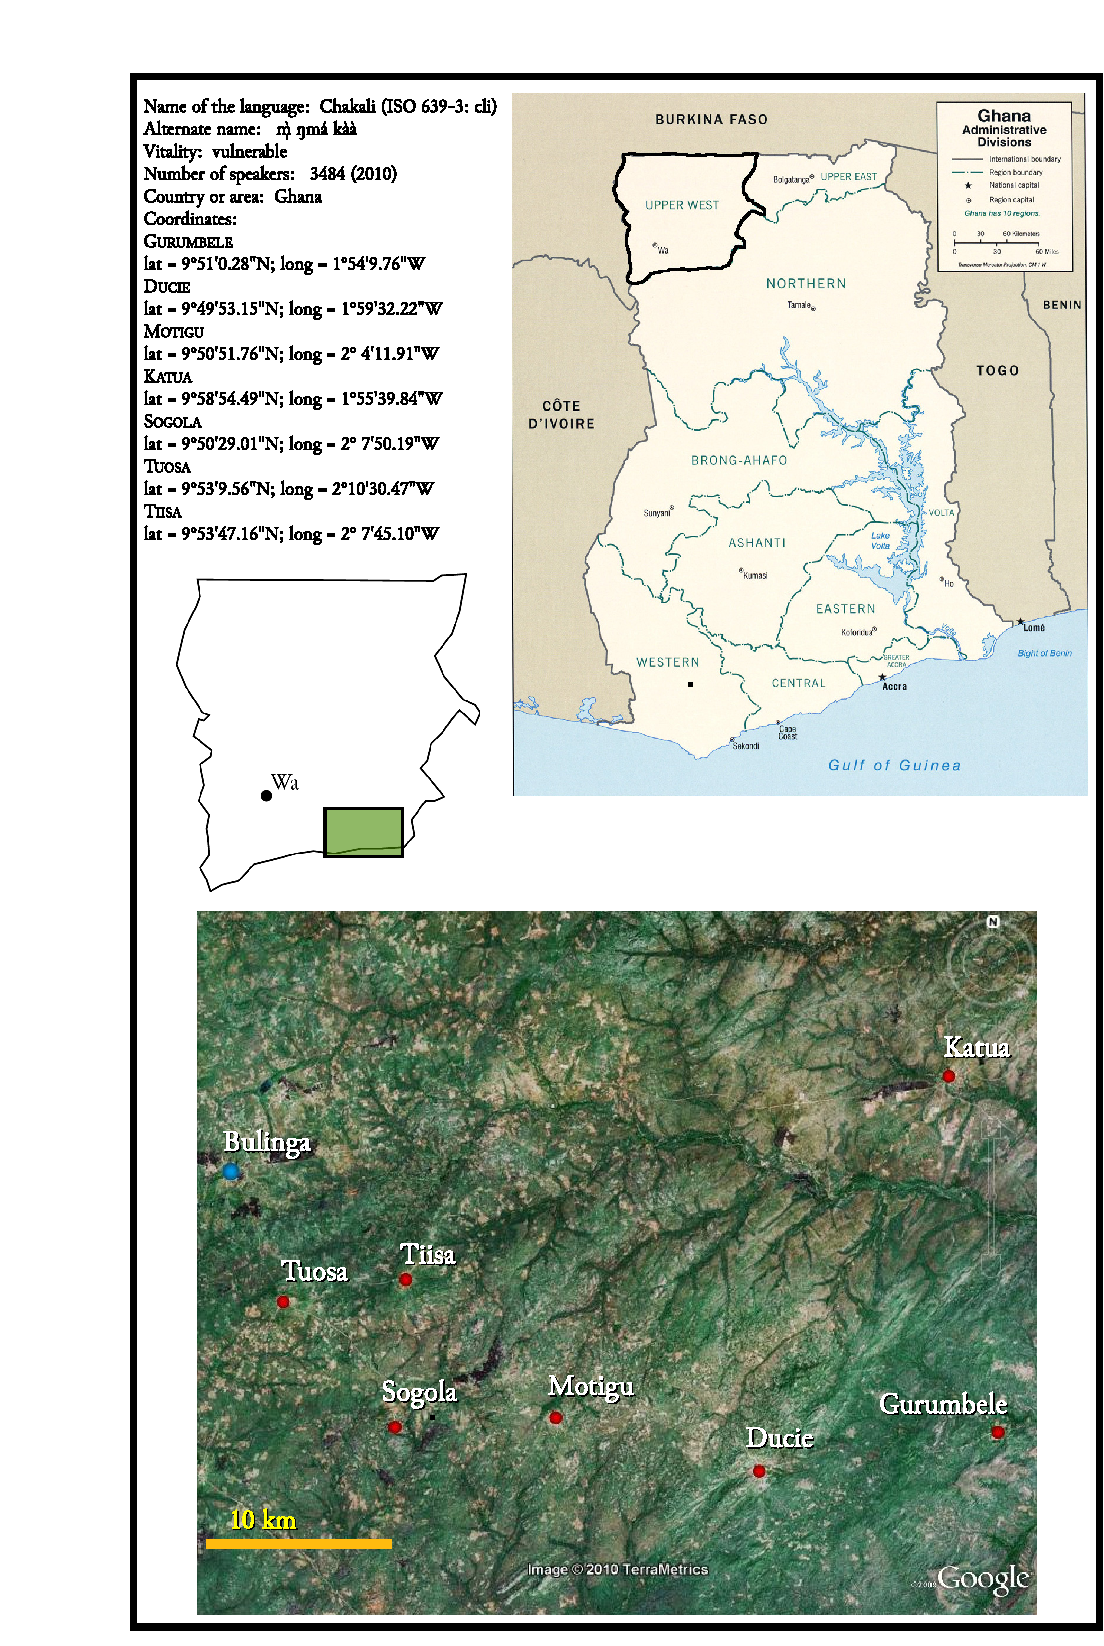
\includegraphics[height=7.2in]{Graphic/Maps/climapII.pdf}
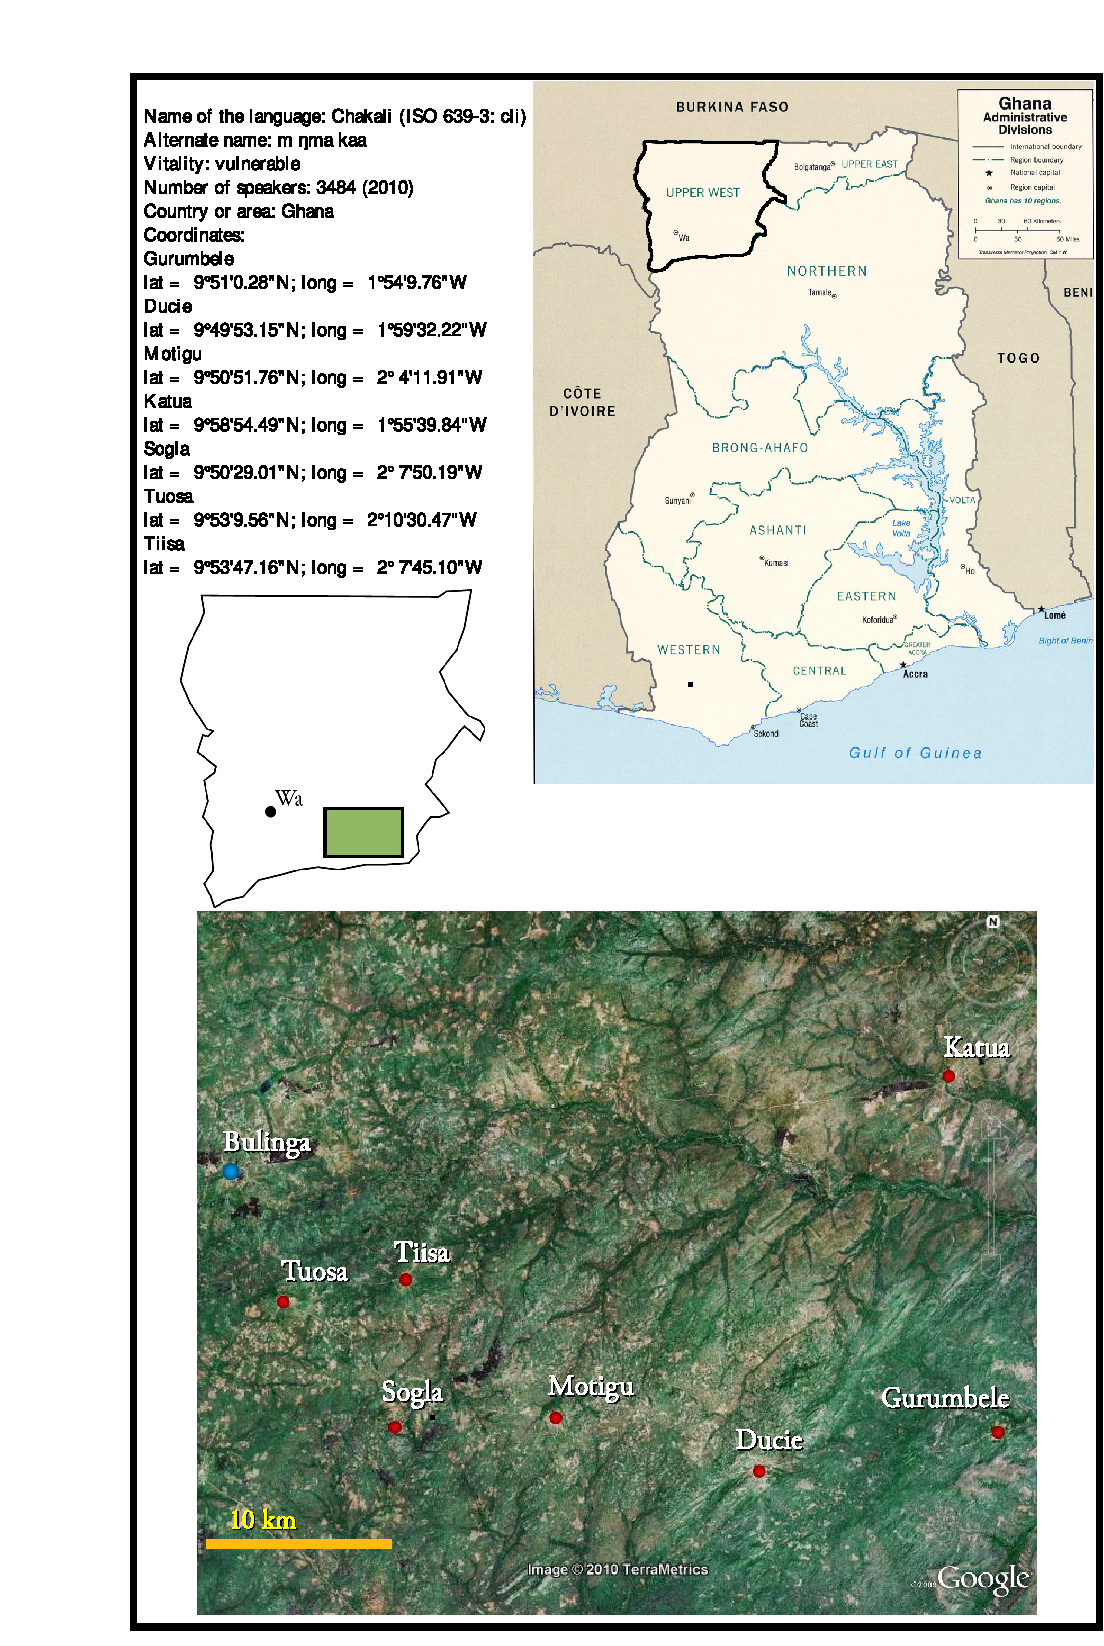
\includegraphics[clip=true, trim= 20mm 0mm 0mm 10mm, 
height=7.2in]{Graphic/Maps/climap.pdf}
% climap.pdf: 0x0 pixel, 0dpi, 0.00x0.00 cm, bb=

\caption[Chakali speaking area]{Chakali
speaking villages (Gurumbele,
Ducie, Motigu, Sogla, Tuosa, Tiisa and  Katua), Bulenga and Upper West
 regional capital Wa (Source: Google\texttrademark \   and Central Intelligence
Agency) \label{fig:INT-cliland}}
\end{figure}



% We have been granted the right  to present the data by the  landlords
% and the council of  elders in Ducie and Gurumbele (see \ref{}
% for a copy of the informed consent).




%Method: difference between establishing data and analyse the data (quantity and
%quality advantage and disadvantage of each)- deductive vs. inductive and
%theoretical vs. empirical. Blurred both quantitative for the phonology and
%lexicon chapter and qualitative for the "extensive" chapters. inductive:
%necessarily lead to a conclusion, no preestablished hypotheses deductive:
%relevance theory 
%Theory driven (theoretical) and data driven (empirical): it's harder to be
%empirical and deductive 





%\pagebreak